% !Mode:: "TeX:UTF-8"
%%% Local Variables:
%%% mode: latex
%%% TeX-master: t
%%% End:

%面向对象的遥感影像的区间二型模糊聚类分割算法
\chapter{基于CGAN 影像分类的改进方法}
\label{cha:chap04}

\section{引言}
\label{sec:chap04-1}
在第~\ref{cha:chap03} 章中,我们将对抗训练的思想应用到FCN 分类模型中,提出了基于CGAN 影像分类方法。模型的对抗损失一定程度上增强了影像像素点间的连续性,提高了FCN 方法的影像分类效果。然而,因为遥感数据固有的不确定性,相比自然图像,遥感影像分类地物边界混淆、歧义性较严重。此外,模型中反卷积上采样操作将特征图恢复到原始影像尺寸,特征的损失也加剧了地物分类的边界模糊问题。因此,本章试图从影像边界信息补充和分割结果后处理两个角度改进基于CGAN 的遥感影像分类方法。本文作者于2017年研究过高分影像数据不确定性特征处理相关的内容,提出一种基于三角形模糊集值的区间二型模糊聚类方法(Triangular Fuzzy Set Valued Interval Type 2 Fuzzy Clustering Method, TFSV-IT2FCM) 方法\cite{jiang2018enhanced} 用于区分高分影像地物边界。并取得了较好的效果,因此尝试将影像不确定性数据特征的提取结果作为CGAN 分割模型的预处理知识,用于改进基于CGAN 影像分类方法的精度。


\section{TFSV-IT2FCM 聚类分割}
\label{sec:chap04-2}

\subsection{方法原理}
\label{subsec:chap04-2-1}
由于遥感影像数据存在不确定性和混合边界问题,模糊C均值聚类(Fuzzy c-means clustering, FCM)方法被广泛应用到遥感影像解译中\cite{bezdek1984fcm}。随着高分影像数据的普及,遥感影像模糊聚类方法由基于像元的聚类方法发展为面向对象的模糊聚类方法。本文作者提出的TFSV-IT2FCM 方法就是面向对象的高分影像模糊聚类分割方法。TFSV-IT2FCM 算法首先定义三角形模糊集数据模型(Triangular Fuzzy Set Valued, TFSV)对高分影像的分割单元建模,能够表征影像分割单元内的像素点特征。然后定义一种新的区间值距离来度量两个TSFV 数的相似性。最后基于TFSV 数据模型和新的距离度量提出TFSV-ITFCM 模糊聚类方法。TFSV-ITFCM 聚类分割结果为许多同质性的聚类簇。各聚类簇的像素点差异性不大,且对簇内像素点变化具有一定容忍度。即某一簇内的所有像素点可视作同类地物。

\begin{figure}[!h]
    \centering
    \includegraphics[width=0.9\textwidth]{figures/tfsvit2fcm}
    \caption{TFSV-IT2FCM 算法框架}
    \label{fig:tfsvit2fcm}
\end{figure}

TFSV-IT2FCM 方法的整体框架如图\ref{fig:tfsvit2fcm} 所示。首先对高分影像$\bm{I}$ ,使用SLIC 分割算法获得影像分割单元 $\bm{SS}$,为:
\begin{equation}\label{eq:image_ss}
    \begin{split}
        \bm{SS} = \lbrace \bm{B_1}, \bm{B_2},\bm{\cdots}, \bm{B_n} \rbrace
    \end{split}
\end{equation}
其中$\bm{B_i}(1 \leq i \leq n)$ 表示第$i$ 个分割单元,$n$ 表示分割单元的总数。 $\bm{B_i}(i=1,2,\cdots, n)$ 是一个$j \times p$ 矩阵,其中$j$ 表示每个波段包含的像素数目,$p$ 表示图像通道数。对任一个影像单元$\bm{B_i}$ 均可以定义为一个TFSV 数据模型$\bm{\tilde{A_i}}$,影像分割单元的数据不确定性特征可由$\bm{\tilde{A_i}}$表达。即影像所有分割单元集合$\bm{SS} = \lbrace \bm{B_1}, \bm{B_2},\bm{\cdots}, \bm{B_n} \rbrace$ 可以被表示为:

\begin{equation}\label{eq:eq-2}
    \bm{SS} \to \lbrace \bm{\tilde{A_1}}, \bm{\tilde{A_2}},\bm{\cdots}, \bm{\tilde{A_n}} \rbrace
\end{equation}
其中$\bm{SS}$ 是一个$n \times p$ 矩阵,$\bm{\tilde{A_i}}$ 是$\bm{B_i}$ 对应的$p$ 维TFSV 数据,$n$ 表示分割单元的数目。$d_I$ 是定义TFSV 数据模型间的区间值距离,对于两个TFSV 数据$\tilde{A}$ 和$\tilde{B}$ 的区间值距离$d_I (\tilde{A}, \tilde{B})$ 为下式:
\begin{equation}\label{eq:interval}
    \begin{split}
        d _{I} (\tilde{A},\tilde{B}) = [\min \lbrace d_0 (\tilde{A},\tilde{B}),d_1(\tilde{A},\tilde{B}) \rbrace, \max \lbrace d_0(\tilde{A},\tilde{B}), d_1 (\tilde{A},\tilde{B}) \rbrace ]
    \end{split}
\end{equation}
式中$d_0 (\tilde{A},\tilde{B})$ 和$d_1 (\tilde{A},\tilde{B})$ 分别为$\tilde{A}$ 和$\tilde{B}$ 的$0 − cut$ 和$ 1 − cut$ 豪斯多夫距离\cite{zadeh1978fuzzy}。区间二型模糊聚类模型的隶属度上界$\overline{u}_{ij}$ 和下界$\underline{u}_{ij}$隶属度则由区间值距离$d _{I} $ 和模糊指数$m$ 求解,分别为:
\begin{equation}\label{eq:13}
    \begin{split}
        \overline{u}_{ij} = \max \Bigg \lbrace \frac{1}{\sum_{k=1}^K {(\frac{d_{ji}^0}{d_{ki}^0})}^{\frac{2}{m-1}}}, \frac{1}{\sum_{k=1}^K {(\frac{d_{ji}^1}{d_{ki}^1})}^{\frac{2}{m-1}}} \Bigg \rbrace
    \end{split}
\end{equation}
和
\begin{equation}\label{eq:14}
    \begin{split}
        \underline{u}_{ij} = \min \Bigg \lbrace \frac{1}{\sum_{k=1}^K {(\frac{d_{ji}^0}{d_{ki}^0})}^{\frac{2}{m-1}}}, \frac{1}{\sum_{k=1}^K {(\frac{d_{ji}^1}{d_{ki}^1})}^{\frac{2}{m-1}}} \Bigg \rbrace
    \end{split}
\end{equation}
其中$d_{ji}^0$ 和$d_{ji}^1$ 分别是输入样本$\tilde{X_i}$ 和聚类中心$\tilde{V_j}$ 的$0-cut$ 距离和$1-cut$ 距离度量,由区间值距离$d_{I} (\tilde{X_i}, \tilde{V_j})$ 计算得出。聚类迭代更新,求解区间二型的模糊划分矩阵$\bm{U} = [U_{ij}]_{n \times K}$
\begin{equation}\label{eq:21}
    U_{ij} = \frac{\underline{u}_{ij} + \overline{u}_{ij}}{2}
\end{equation}
其中 $U_{ij} = [\underline{u}_{ij}, \overline{u}_{ij}]$。然后,求出$\bm{\tilde{X}_i}$ 到聚类中心$\bm{\tilde{V}_k}$ 的最大隶属度$U_{ik}$ ,其中$k = 1, 2,\cdots, K$。最后根据最大隶属度原则,将$\bm{\tilde{X}_i}$ 划分到类别$\bm{\tilde{V}_k}$, 完成TFSV-IT2FCM 聚类分割过程。

TFSV-IT2FCM 聚类分割方法可以看作是邻域内同质性像素点关系的建模,即邻域内具有相近像素值的像素点将被划分为同一个类别。同时,因模糊不确定度量的存在,同个聚类簇内的像素点可以在一定范围内波动。将TFSV-IT2FCM 聚类分割方法作用到高分影像,可以将各类别地物划分为不同的分类簇,而同一个簇内的像素点基本隶属于同一个地物类别,邻近簇之间的边界也有机率为相邻的不同地物类别的分类边界(也可能是同类地物的,当地物内部差异巨大时,同一地物会被模糊聚类为多个簇)。

\subsection{影像数据处理}
\label{subsec:chap04-2-2}
第\ref{cha:chap03} 章实验用到的Vaihingen 数据为$16$ 张尺寸约为$ 2563 \times 2049$ 的高分影像。为了提取影像整体的辅助边界信息,这里直接使用TFSV-IT2FCM 聚类分割方法分别对这$16$ 张大尺寸影像聚类分割。因Vaihingen 数据共有地面、低矮植被、树木、建筑物、车辆、背景这六类地物,故TFSV-IT2FCM 聚类分割中聚类数为六类。

\begin{figure}[!h]
    \centering
    \includegraphics[width=1.0\textwidth]{figures/tfsv_seg}
    \caption{TFSV-IT2FCM 提取Vaihingen影像辅助特征信息}
    \label{fig:tfsv_seg}
\end{figure}

图\ref{fig:tfsv_seg} 为TFSV-IT2FCM 方法提取Vaihingen影像辅助信息结果图。图\ref{fig:tfsv_seg}(a) 为Vaihingen 数据标号为$30$ 的影像,该影像尺寸为$1983\times2556$。使用TFSV-IT2FCM 聚类方法对影像进行分割,可以将影像依据分割单元的同质近似性,划分为许多个大小不一的簇,分割簇内的点输出标签相同,相邻簇间输出标签不同,图\ref{fig:tfsv_seg}(b) 即为影像聚类分割结果(聚类结果为一个波段二维矩阵,这里可视化三通道RGB 彩色图像),从聚类结果图上我们很容易获取各个簇之间的边界信息,依据TFSV-IT2FCM 聚类分割结果提取到的影像边界信息如图\ref{fig:tfsv_seg}(c) 所示。 图\ref{fig:tfsv_seg}(d)为影响中间某区域的放大展示结果。

类似上面的处理方法,对Vaihingen 数据集内所有的$16$ 张影像均进行TFSV-IT2FCM 聚类分割操作,得到影像的分割单元的边界和簇内点相同标签的辅助信息。数据聚类分割结果为二维的类别矩阵,这里将标签值采用最大最小归一化方法映射到$[0,1]$区间范围内。经过TFSV-IT2FCM聚类分割方法得到的影像边界辅助信息图与原始影像尺寸相同,且位置坐标一一对应。在第\ref{cha:chap03} 章随机滑动窗口裁切原始影像获取大小为$256\times 256$ 的训练样本时,也按照相同的滑窗裁切方式对同区域的影像辅助分割图进行裁切,得到训练样本边界辅助信息图。同理,待测试影像在按照规则网格裁切影像获取测试样本时也对测试影像的影像辅助分割图进行裁切。确保数据集所有样本同一区域的影像数据、类别标签图和经TFSV-IT2FCM 方法得到的影像辅助分割信息图三者一致对应。此外,利用TFSV-IT2FCM 方法获取影像辅助特征属于数据初始处理阶段,不会增加CGAN 模型的迭代训练时间。


\section{带有先验边界辅助信息的CGAN 影像分类方法}
\label{sec::chap04-4}

在上一小节中,我们使用TFSV-IT2FCM 聚类分割方法对高分影像数据做无监督聚类分割处理,通过模型中的TFSV 模型对影像数据不确定性建模,聚类过程将影像划分为多个大小不一的分类簇。同一个分割单元簇内像素具有较强的类别一致性,簇之间的分割边界则有可能为异类地物的分割边界。对模型中所有的训练样本和测试样本均获得影像聚类分割的辅助特征信息图。

第\ref{cha:chap03}章中基于CGAN 的影像分类方法使用正射影像和DSM 数据组成的四波段融合数据作为模型输入,能够得到最好的影像分类结果。这里,将聚类分割的辅助特征信息图作为影像新波段数据,融合到CGAN 模型样本中。


\section{基于辅助信息后处理的影像分类方法}
\label{sec::chap04-4}
上一节中我们将聚类分割得到的边界辅助特征信息作为一个新波段加入模型训练数据中,从一定程度上能够增加影像一定空间范围内像素点之间的相互关系。然而,在分割模型小尺寸特征图反卷积上采样恢复原始影像尺寸的过程中,特征图边界信息的损失难以避免。此外,分割模型最后一层输出的是影像各像素点所属类别的概率分布。像素点的预测分类没有考虑邻域像素点间关系。容易导致分类结果中出现很多细碎的错分区域。借鉴FCN 模型中跳跃连接弥补特征损失的思想,我们将上一节通过TFSV-IT2FCM 聚类方法得到的辅助分割信息图特征应用到分割模型输出层中,分类预测时考虑单个像素分类概率值和辅助分割信息图中同一分割单元内其他像素点的相互关系,优化分类图像中粗糙和不确定的像素的预测标签。这样既可减少同类地物中细碎的错分问题,同时又可以得到更精细、准确的地物分割边界。




\section{实验结果与分析}
\label{sec::chap04-5}

\begin{table*}[!h]
    \centering
    \caption{各优化方法影像分类精度表}\label{tab:gaijin_cgan}
    \resizebox{\textwidth}{!}{
        \begin{threeparttable}[b]
            \begin{tabular}{ccccccccc}
                \toprule
                方法                        & 地面      & 低矮植被  & 树木      & 建筑物    & 车辆      & OA        & mIoU               \\
                \midrule
                CGAN                        & $83.78\%$ & $74.47\%$ & $82.40\%$ & $87.64\%$ & $78.83\%$ & $80.15\%$ & \textbf{$61.83\%$} \\
                辅助特征 + CGAN         & $83.78\%$ & $74.47\%$ & $82.40\%$ & $87.64\%$ & $78.83\%$ & $80.15\%$ & \textbf{$61.83\%$} \\
                CGAN + 后处理               & $83.78\%$ & $74.47\%$ & $82.40\%$ & $87.64\%$ & $78.83\%$ & $80.15\%$ & \textbf{$61.83\%$} \\
                辅助特征+ CGAN + 后处理 & $83.78\%$ & $74.47\%$ & $82.40\%$ & $87.64\%$ & $78.83\%$ & $80.15\%$ & \textbf{$61.83\%$} \\
                辅助特征+ FCN + 后处理  & $81.14\%$ & $63.39\%$ & $79.52\%$ & $83.96\%$ & $62.39\%$ & $78.48\%$ & $58.42\%$          \\
                \bottomrule
            \end{tabular}
        \end{threeparttable}
    }
\end{table*}


神湾研究是一个复杂的种植区域,该区域的高分影像由SPOT 5 遥感卫星于2008 年拍摄。SPOT 5遥感卫星影像包含四个波段,空间分辨率大约$10$ 米,光谱范围$0.4-0.9$ 微米。 神湾地区地物覆被可划分为5大类,分别是:水域、草地、建筑和养殖水域。实验中选择影像$B1$、$B2$、$B3$ 波段合成RGB 图像,如图\ref{fig:hengqin}(a) 所示,其包含$400 \times 400$ 个像素。

在该研究区,文中提出的面向对象的TFSV-IT2FCM 算法分别与其他聚类分割算法进行比较,包含基于像素的聚类方法 (FCM 算法,IT2FCM 算法)和面向对象的聚类方法 (面向对象的IT2FCM, 面向对象的基于CGAN 的方法 算法),聚类结果分别由图\ref{fig:hengqin}(f)-(i) 展示。另外,文中提出的TFSV-IT2FCM 算法包含三个主要处理步骤:影像分割,聚类和后处理。图\ref{fig:hengqin}(c) 和\ref{fig:hengqin}(d) 分别展示是否使用后处理的分割结果;图\ref{fig:hengqin}(e) 是获取影像分割单元时使用分水岭分割算法替换SLIC 超像素分割算法得到。通过目视各方法对研究区的聚类分割结果,可以得到以下结论:

\begin{enumerate}[(1)]
    \item 图\ref{fig:hengqin}(c) 和\ref{fig:hengqin}(d) 无论是否使用后处理操作,两者均有大致相似的分割类别区域,图\ref{fig:hengqin}(d) 使用后处理操作具有较少的奇异点。
    \item 图\ref{fig:hengqin}(e) 中使用分水岭算法获取分割单元,与图\ref{fig:hengqin}(d) 相比,一些建筑类别的分割单元被错误划分为草地。因此,获取影像分割单元的分割算法在一定程度上会影像最后聚类分割的精度。
    \item 比较图\ref{fig:hengqin}(f)-(i) 和图\ref{fig:hengqin}(d) 中的聚类计结果可知,这些聚类方法在水域的识别上都有不错的效果。然而,对于基于CGAN 的方法 算法(图\ref{fig:hengqin}(f)),一些草地类别被错分为林地类别;对于面向对象的IT2FCM 算法(图\ref{fig:hengqin}(g)),由于建筑、草地和林地这三类有相近的光谱波段,图中左下角区域无法明确区分三者;另外,与面向对象的方法相比,基于像素的IT2FCM 算法和FCM 算法(分别为图\ref{fig:hengqin}(g) 和(h)) 在同类别大区域中产生许多异类别的异常小块。
\end{enumerate}
综上所述,神湾研究区可视化的分类结果图表明文中提出的TFSV-IT2FCM 聚类分割算法相比其他已有算法能获得更好的遥感影像分割结果。


为了得到实验中精确量化的聚类结果图,实验中使用CORINE 土地覆被分类系统生成地物类别ground truth 图,如图\ref{fig:hengqin}(b) 所示。表~\ref{tab:shenwan_data} 为神湾研究区各类别地物抽样点数据表。为了对分类结果进行评价,确定分类的精度和可靠性。本实验中使用以下评价指标度量分类效果:
\begin{enumerate}
    \item \textbf{总体分类精度(Overall accuracy, OA)}

          总体分类精度是指所有类别中正确分类的像元总和除以总像元数。
    \item \textbf{Kappa 系数}

          Kappa 系数基于混淆矩阵,用于衡量分类精度。计算公式为
          \begin{equation}\label{eq:kappa}
              \begin{split}
                  Kappa = \frac{\mbox{总体准确度}-\mbox{期望准确度}}{1-\mbox{期望准确度}} = \frac{N\sum_{i=1}^n(X_{ii}) - \sum_{i=1}^n(X_{i+} \times X_{+i})}{N^2 - \sum_{i=1}^n(X_{i+} \times X_{+i})}
              \end{split}
          \end{equation}
\end{enumerate}
式中,$n$ 表示类别,$N$ 表示总类别数,$X_{ii}$ 表示混淆矩阵对角线元素,$X_{+i}$ 表示类别的行总和,$X_{i+}$ 表示类别的列总和。


\begin{table}[htb]
    \caption{影像地物类别抽样Ground truth表(pixels)}\label{tab:shenwan_data}
    \centering
    \begin{tabular}{ccccc}
        \toprule
        林地  & 水域  & 草地  & 建筑  & 养殖水域 \\
        \midrule
        10124 & 46250 & 15687 & 23697 & 6942     \\
        \bottomrule
    \end{tabular}
\end{table}


表~\ref{tab:shenwan_result} 为各方法在神湾地区影像上的地物类别识别精度。文中提出的TFSV-IT2FCM 算法获得最好的OA 精度,为$90.33\%$,相比无后处理的TFSV-IT2FCM 算法、基于Watershed 分割的TFSV-IT2FCM 算法、 基于CGAN 的方法 算法、面向对象的IT2FCM 算法、基于像素的IT2FCM 算法和FCM 算法分别提升了$0.55\%$、$0.52\%$、$2.22\%$、$4.81\%$、$5.43\%$的分类精度。
分类精度也表明对于文中提出的聚类分割算法,聚类是最重要的一步,在方法的三个部分(分割、聚类、后处理)中最大化的决定最终分类结果精度。Kappa系数结果也表明,文中提出的TFSV-IT2FCM 算法有效题目了影像地物的特征,获得了最佳的聚类分割结果。表中数值量化的结果基本与前文可视化的结果一致。

\begin{figure}[htbp]
    \centering
    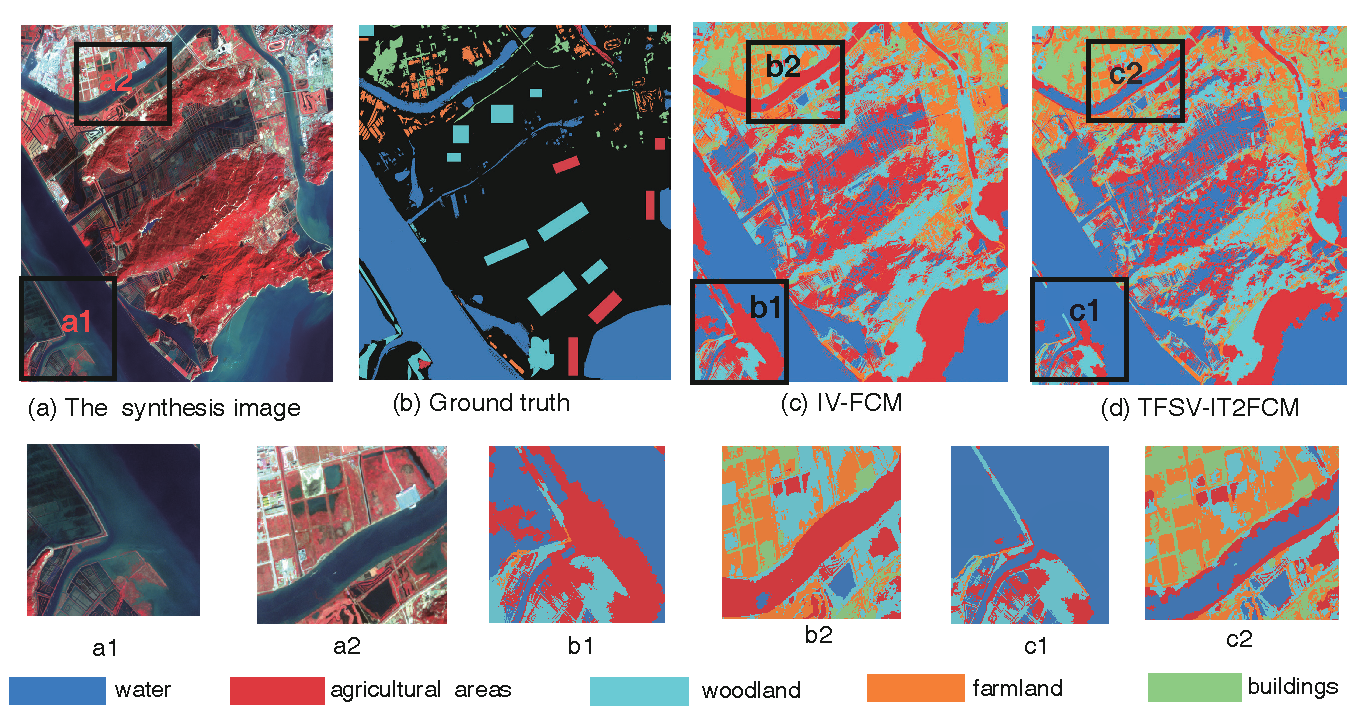
\includegraphics[width=1.0\textwidth]{figures/hengqin}
    \caption{基于CGAN 影像分类后处理方法分割图 }\label{fig:hengqin}
\end{figure}


\begin{table*}[htbp]
    \centering
    \caption{ 基于CGAN 影像分类后处理方法的精度表}
    \label{tab:shenwan_result}
    \resizebox{\textwidth}{!}{
        \begin{threeparttable}[b]
            \begin{tabular}{cccccccc}
                \toprule
                地物类别                   & TFSV-IT2FCM\tnote{1} & TFSV-IT2FCM\tnote & TFSV-IT2FCM\tnote{2} & 基于CGAN 的方法 & IT2FCM\tnote{2} & IT2FCM\tnote{4} & FCM    \\\cline{1-8}
                \multicolumn{8}{c}{生产者精度 (\%)}                                                                                                                         \\
                \midrule
                林地                       & 89.39                & 89.44             & 89.44                & 89.52           & 79.70           & 89.32           & 79.70  \\
                水域                       & 94.08                & 94.58             & 94.18                & 93.59           & 94.06           & 94.09           & 94.21  \\
                草地                       & 83.69                & 84.23             & 84.78                & 79.74           & 81.28           & 77.91           & 80.43  \\
                建筑                       & 87.88                & 88.45             & 88.14                & 88.21           & 87.73           & 83.58           & 81.00  \\
                养殖水域                   & 80.32                & 81.29             & 76.01                & 64.08           & 50.83           & 48.33           & 45.73  \\\cline{1-8}
                \multicolumn{8}{c}{用户精度 (\%)}                                                                                                                           \\\cline{1-8}
                林地                       & 82.98                & 83.39             & 83.39                & 84.10           & 77.46           & 82.40           & 77.46  \\
                水域                       & 95.54                & 97.34             & 97.34                & 97.34           & 95.18           & 92.58           & 90.85  \\
                草地                       & 82.96                & 82.96             & 82.96                & 80.69           & 70.21           & 72.32           & 63.84  \\
                建筑                       & 91.95                & 90.68             & 87.97                & 86.04           & 84.60           & 86.04           & 86.46  \\
                养殖水域                   & 69.27                & 69.27             & 70.71                & 56.31           & 70.71           & 61.93           & 69.27  \\
                \cline{1-8}
                \textbf{总体分类精度 (\%)} & 89.78                & 90.33             & 89.81                & 88.11           & 85.52           & 84.90           & 82.93  \\
                \textbf{Kappa 系数}        & 0.8544               & 0.8621            & 0.8546               & 0.8302          & 0.7954          & 0.7871          & 0.7605 \\
                \bottomrule
            \end{tabular}
            \begin{tablenotes}
                \item[1] {TFSV-IT2FCM 算法,没有做后处理}
                \item[2]{该方法中影像分割阶段使用Watershed 方法获取影像分割单元}
                \item[3]{面向对象的IT2FCM 方法}
                \item[4]{基于像素的IT2FCM 方法}
            \end{tablenotes}
        \end{threeparttable}
    }
\end{table*}

第二个研究区横琴岛位于广东省珠海市,岛内具有复杂的农业与养殖区,该区域高分影像
由SPOT 5 遥感卫星于2010 年拍摄。横琴地区地物类别可分为水域、农业区、林地、农田和建筑这五大类。实验区选择影像图像如图~\ref{fig:hengqin}(a) 所示,大小为$1203 \times 1055$ 个像素。

在神湾研究区我们比较了文中提出的TFSV-IT2FCM 算法与其他算法的聚类分割结果,初步验证了TFSV-IT2FCM 算法的改进效果。文献\cite{he2016remote} 中证明了基于CGAN 的方法 算法相比其他聚类分割算法可以取得更好的实验精度,因此,在横琴地区和三门峡地区的实验中,我们着重比较提出的TFSV-IT2FCM 算法与基于CGAN 的方法 算法的实验效果。

基于CGAN 的方法 算法和TFSV-IT2FCM 算法的可视化结果分别如图~\ref{fig:hengqin}(c) 和(d) 所示。结合目视解译可知,两种方法对具有明显边界的地物类别都有良好的划分,基本实现同一类地物划分的一致性。 参照图~\ref{fig:hengqin}(b) 中的真实地物分类,对比~\ref{fig:hengqin}(c) 和(d)中可视化结果,可以看出TFSV-IT2FCM算法对于一定范围内不同光谱特征的同一类别具有较大的容忍性。例如,图~\ref{fig:hengqin}(a1) 左上角水域的光谱特征是不均匀的,图~\ref{fig:hengqin}(b1) 和(c1) 结果表明TFSV-IT2FCM 算法将该区域正确划分为水域,由于水域的几个光谱与农业区相近,而基于CGAN 的方法 算法则将其错分为农业区。类似地,对于图~\ref{fig:hengqin}(a2)中地物覆被复杂的区域,TFSV-IT2FCM 算法能正确地将水与农田、建筑物等其他地物区分开来,而基于CGAN 的方法 算法则存在一定的分类错误。例如,在图~\ref{fig:hengqin}(b2)中,河流中的水被错误地划分为农业区; 然而,在图~\ref{fig:hengqin}(c2)中,TFSV-IT2FCM算法的结果清晰地识别出了河流两岸的水和其他物体。



同样,为了获取横琴地区精确的分类结果,文中使用CORINE 土地分类系统随机采样$499,669$ 个像素点作为ground truth 图,如表~\ref{tab:shenwan_result} 所示,TFSV-IT2FCM 方法中$10,022$ 个像素由“农业区” 被错分为“水域”,而在基于CGAN 的方法 方法中被错分的像素点为$54,380$ 个。TFSV-IT2FCM 方法相比基于CGAN 的方法 方法,“水域”类别的用户精度从$78.12\%$ 提升到$95.99\%$。 表~\ref{tab:shenwan_result} 中的用户精度和生产者精度也表明TFSV-IT2FCM 聚类方法的性能要比基于CGAN 的方法 方法更好。

\begin{table}[htbp]
    \caption{带有边界辅助信息分类精度表}\label{tab:hengqin_oa}
    \centering
    \begin{tabular}{llll}
        \toprule
        研究区 & 方法            & OA(\%) & Kappa 系数 \\
        \midrule
        横琴   & TFSV-IT2FCM     & 88.63  & 0.8290     \\
               & 基于CGAN 的方法 & 80.49  & 0.7210     \\
        \bottomrule
    \end{tabular}
\end{table}

表~\ref{tab:hengqin_oa} 中比较了TFSV-IT2FCM 方法和基于CGAN 的方法 方法在横琴地区的总体分类精度和Kappa 系数,TFSV-IT2FCM 方法的OA 从$80.49\%$ 提升到$88.63\%$, 同时Kappa 系数由$0.7210$ 提升到$0.8290$。



\section{本章小结}
\label{sec::chap04-6}
本章从遥感影像不确定性特征表达角度展开研究,TFSV-IT2FCM 分割影像提取影像分割单元内在特征信息,从影像边界信息补充和分割结果后处理两个角度改进基于CGAN 的遥感影像分类方法,实验验证其确实能更好刻画遥感影像数据的不确定性,实现更好的分割识别结果。%改进现有面向对象的遥感影像模糊聚类分割方法。
